\section{Durchführung}
\label{sec:Durchführung}
Die Trägheitsmomente von zwei Körpern, sowie einer Puppe, werden mithilfe
einer Drillachse bestimmt. Dazu werden die Körper auf einer drehbaren Achse befestigt,
welche über eine Spiralfeder mit einem Rahmen verbunden ist. Zunächst wird eine Federwaage
in einen Haken eingehängt. Die Federwaage muss dabei möglichst senkrecht zur Drehachse
und zum Radius der Kreisbahn der schwingenden Körper gehalten werden, da
die Federwaage sonst eine ungenauere Kraft anzeigt.
\begin{equation}
  M = |\symbf{r} \times \symbf{F}| = r F sin(\theta)
\end{equation}
$sin(\theta)$ ist bei einem 90° Winkel maximal. Die Federwaage wird für 10 unterschiedliche
Winkel ausgelenkt und die zugehörige Kraft von der Federwaage abgelesen.

\begin{figure}[H]
  \centering
  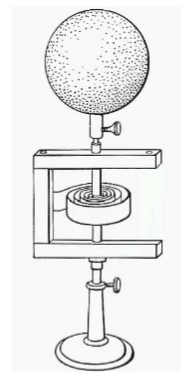
\includegraphics[height=8cm]{Drillachse.PNG}
  \caption{Die Drillachse.}
  \label{fig:drill}
\end{figure}

Eine als masselos angenommene Stange wird auf der Drehachse befestigt. An beiden
Seiten werden Gewichte angebracht und das System wird ausgelenkt und in Schwingung
versetzt, wobei die Periodendauer $T$ der Schwingung gemessen wird. Dieser Vorgang
wird 10 mal für verschiedene Abstände $a$ der Gewichte zum Mittelpunkt durchgeführt.

Ein Zylinder und eine Kugel werden nacheinander auf der Drillachse befestigt und
in Schwingung versetzt. Es wird die Periodendauer $T$ für jeweils 5 Auslenkungen
aus der Ruhelage mit einer Stoppuhr gemessen.

Die Periodendauer einer Holzpuppe wird analog bestimmt. Die Holzpuppe
hat für die ersten 5 Messungen angelehnte Arme und Beine. Bei den nächsten 5
Messungen sind ihre Arme ausgestreckt und ihre Beine angelehnt.
